\documentclass[12pt]{article}
\usepackage[utf8]{inputenc}
\usepackage[T2A]{fontenc}
\usepackage[russian]{babel}
\usepackage{amsmath}
\usepackage{amssymb}
\usepackage{dsfont}
\usepackage[dvipsnames]{xcolor}
\usepackage{setspace}
\usepackage{multirow}
\usepackage[a4paper, outer=1.5cm, inner=1.5cm, top=1cm, bottom=1cm]{geometry}
\usepackage{graphicx}
\usepackage{skull}
\usepackage{wasysym}
\usepackage{float}
\graphicspath{{.images/}}
\usepackage{hyperref}
\hypersetup{colorlinks=true, linkcolor=blue, filecolor=magenta, urlcolor=cyan}
\usepackage[firstpage]{draftwatermark}
\SetWatermarkText{
    $\qquad\qquad\qquad\qquad\qquad$\parbox{7cm}{\begin{center}
    
\includegraphics[width = 0.08\textwidth]{lion-logo.png}\bigskip\\~\bigskip\\~\vspace{-24mm}\\~\end{center}}
}
\SetWatermarkAngle{0}
\SetWatermarkScale{1.5}
\usepackage{etoolbox}

\newtoggle{ifsolved}
\newtoggle{needhelp}
\newcounter{num}
\setcounter{num}{1}

\newcommand{\newnum}{\par\textbf{\textnumero\arabic{num}}\stepcounter{num}}
\newcommand{\sol}{\vspace{3mm}\par\textbf{Решение: }}
\newcommand{\ans}{\vspace{3mm}\par\textbf{Ответ: }}
\newcommand{\hint}{\vspace{3mm}\par\textbf{Подсказка: }}
\newcommand{\mode}[1]{
\ifstrequal{#1}{0}{\togglefalse{ifsolved}\togglefalse{needhelp}}{\ifstrequal{#1}{1}{\togglefalse{ifsolved}\toggletrue{needhelp}}{\ifstrequal{#1}{2}{\toggletrue{ifsolved}\togglefalse{needhelp}}{\toggletrue{ifsolved}\toggletrue{needhelp}}}}} %if 0 - if 1 - if 2 - else
%\newenvironment{problem}[8]{%#1, #2, #3
%\parbox{\linewidth}{\vspace{4mm}\ifstrequal{#4}{(лёгкая)}{\newnum\textbf{.}}{\newnum\textbf{*.} } \\ #5}
%\iftoggle{ifsolved}{\sol #6}{}
%\iftoggle{ifsolved}{\ans #7}{}
%\iftoggle{needhelp}{\hint #8}{}}

\newenvironment{problem}[8]{%#1, #2, #3
\parbox{\linewidth}{\vspace{5mm}\ifstrequal{#4}{(лёгкая)}{\newnum\textbf{.}}{\newnum\textbf{*.} } \\ #5}
\iftoggle{ifsolved}{\sol #6}{}

\iftoggle{ifsolved}{\parbox{\linewidth}{\ans #7}}{}
\iftoggle{needhelp}{\parbox{\linewidth}{\hint #8}}{}}

\newenvironment{mylist} %custom list
{ \begin{itemize}
    \setlength{\itemsep}{0pt}
    \setlength{\parskip}{0pt}
    \setlength{\parsep}{0pt}     }
{ \end{itemize}                  }

\newenvironment{homeass}[1]{\vspace*{-1.5cm}
\iftoggle{ifsolved}{
    \section*{\center{Решение домашнего задания к #1.}}
}{
    \section*{\center{\textcolor{Sepia}{Домашнее задание к #1}}}
} \vspace{7mm}\large}

\parindent=0pt
\pagestyle{empty}
%$\!$[\arabic{class}.\arabic{num}]
%\ifnumcomp{\value{counter}}{>}{1}{true}{false}
%\definecolor{Gray}{gray}{0.9}
%\definecolor{mypink}{RGB}{219, 48, 122}
%\newcolumntype{g}{>{\columncolor{Gray}}p{2.8cm}}

\begin{document}
\large
\mode{7}
%0 for problems without hints
%1 for problems + hints
%2 for problems + solutions + answers
%else: show all

{\centering\section*{СПИСОК ЗАДАЧ}}

{\centering\subsection*{\smallskip\\\textcolor{green}{\textbf{Полезные вещи, которые можно и нужно копипастить:}}}}

\subsection*{\textcolor{Emerald}{\textbf{Полезные шпаргалки по LaTeXу:}}}

\textbf{Пример вставки рисунка:}

\begin{minipage}{\linewidth}
    \begin{minipage}{0.54\linewidth}
    см. рисунок справа\\
    Текст к собственно пикче, примерно всегда это либо развёрнутое описание, либо большая часть решения задачи --- стремимся экономить пространство, если это можно сделать.
    \end{minipage}
    \hspace{0.05\linewidth}
    \begin{minipage}{0.4\linewidth}
    \begin{figure}[H] 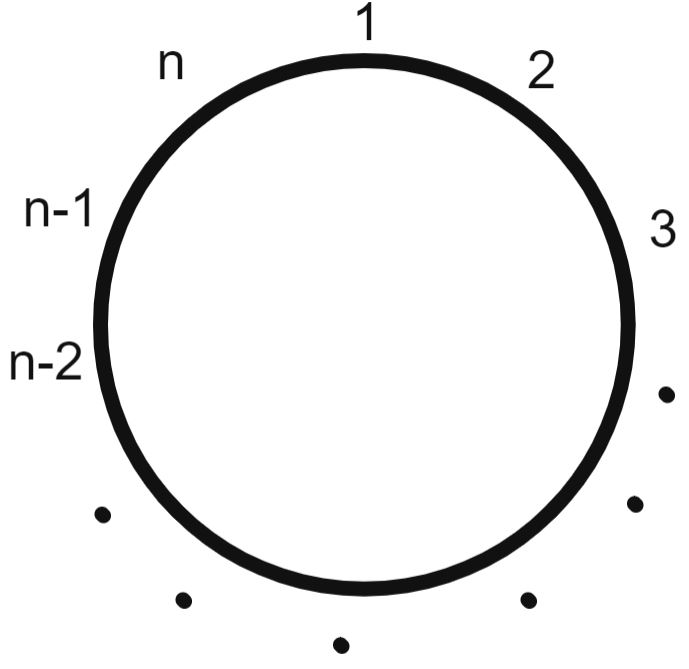
\includegraphics[width=\linewidth]{sol3} %тут поменять имя пикчи
    \end{figure}
    \end{minipage}
\end{minipage}

\textbf{Дефолтные математические знаки и символы:}\\
$\geqslant$,
$\leqslant$,
$a^{b}$,
$x_{i}$,
$\sqrt{a}$,
$\frac{a}{b}$,
$\displaystyle \frac{a}{b}$,
$\cdot$
$\;\Rightarrow\;$,
$\;\Leftrightarrow\;$,
$1{,}2$.
О промежутках:
$a\!b$,
$a\,b$,
$a\:b$,
$a\;b$,
$a\quad b$.

\textbf{Стандартные система и совокупность уравнений / неравенств:}\\
$\left\{
\begin{aligned}
f(x) &= 0 \\
g(x) &= 1
\end{aligned}\right.$

$\left[\begin{aligned}
&\left\{\begin{aligned}
f(x) &\geqslant a \\
g(x) &= b
\end{aligned}\right.\\
&\left\{\begin{aligned}
f(x) &< a \\
g(x) &= -b
\end{aligned}\right.
\end{aligned}\right.$

\subsection*{\textcolor{Emerald}{\textbf{Не математическое, но полезное:}}}
% комментарий в любом месте документа, который нигде не будет видно. Можно использовать для написания заметок-вопросов по задачам
\textbf{Пример таблицы:}

\begin{tabular}{|c|c|c|}
\hline
    $a$ & $b$ & текст
\\\hline
    $c$ & $d$ & мораль
\\\hline
\end{tabular}\\

\textbf{Отступы:} между\smallskip\\ строками\medskip\\ \textbf{Тире} --- это три дефиса.\\
\textbf{Списки:}
\begin{mylist}
\item [$\bullet$] это был пункт а
\item [2)] а это уже пункт номер 2 с изменённым заголовком
\end{mylist}

\subsection*{\textcolor{Emerald}{\textbf{Всё, неупомянутое выше (или если просто что-то не так):}}}
\begin{mylist}
\item [$\bullet$] Решение отдельных вопросов касательно ТеХа нужно искать в \href{https://www.mccme.ru/free-books/llang/newllang.pdf}{Львовском}.

\item [$\bullet$] Найти произвольный символ, который нужен, можно в \href{http://detexify.kirelabs.org/classify.html}{Detexify}.

\item [$\bullet$] Если возникли сомнения при решении, ответ практически ко всем задачам можно проверить с помощью \href{https://www.wolframalpha.com/}{WolframAlpha}.

\item [$\bullet$] Если в задаче нужно создать картинку, то лучше пока отложить эту задачу. Все графики планируется централизованно нарисовать (или перерисовать) в геогебре.

\item [\textcolor{brown}{\textbf{!!}}] Важно ставить \textcolor{red}{\textbf{$\spadesuit$}}
(или просто red) в тело задачи в случае серьёзных вопросов к решению и какой-то вопиющей лажи.

\item [\textcolor{brown}{\textbf{!!}}] Важно ставить \textcolor{olive}{\textbf{$\spadesuit$}}
(или просто olive) в тело задачи в случае не самого удачного текста и кривых отступов.
\end{mylist}

\subsection*{\textcolor{Violet}{\textbf{Комментарии:}}}% а также невидимые комментарии - так можно оставлять заметки-вопросы прямо в задаче, чтобы потом было понятно, в чём вопрос.
\begin{mylist}
\item [$\skull$] Переставлять задачи местами --- очень плохая идея.

\item [$\smiley$] При двойном клике по тексту pdf справа происходит автоматический переход к этому месту в латех-коде, а для обратного перехода можно нажать стрелку вправо (висит сверху между pdf и латех-кодом).

\item [$\smiley$] Если есть размышления, дописывать red/olive к задаче или не дописывать, то лучше всё-таки дописать.

\item [$\skull$] Самое плохое, что можно сделать --- написать в любое поле из трёх (НаписанноеРешение/ВерныйОтвет/Подсказка) только половину того, что надо, никак это не отметить, и потом пойти дальше.\\ Нужно в этот момент писать red/olive в случайном месте задачи, чтобы потом вычислить это с помощью Ctrl+F по всему документу (и это то, что потом будет делаться долго и тщательно)
\end{mylist}

\newpage
\setcounter{num}{1413}

\hypertarget{9.6}{{\centering\section*{\bigskip\\\textcolor{Blue}{\hyperlink{start2}{\textcolor{Blue}{9.6}} Прогрессии.}\vspace{-5mm}}}}

\begin{problem}{Арифметическая прогрессия.}{9.6.2}{7A}{(лёгкая)}
{Чему равно число $1 + 2 + \ldots + 50$?}
{НаписанноеРешение}
{ВерныйОтвет}{Подсказка}
\end{problem}

\begin{problem}{Арифметическая прогрессия.}{9.6.2}{9I}{(лёгкая)}
{Стрелок в тире сделал 30 выстрелов по мишени. Вначале у него было всего 100 баллов, за первое попадание по мишени ему начисляют 5 баллов, за каждое следующее попадание ему начисляют на 5 баллов больше, чем за предыдущее.\\ (если он промахивается, то он получает 0 баллов)\smallskip\\
В конце стрельбы он получает штраф в баллах: $-4 \;\times$ кол-во промахов.
\\a) Сколько раз он промахнулся, если по итогу его счет составил 22 очка?
\\b) Сколько максимум раз можно промахнуться, чтобы сохранить лицо и положительный счет?}
{НаписанноеРешение}
{ВерныйОтвет}{Подсказка}
\end{problem}

\begin{problem}{Геометрическая прогрессия.}{9.6.3}{9I}{(лёгкая)}
{В начале первого года в банк был внесен вклад в размере 2000 рублей. За первый год хранения сумма вклада в банке увеличилась на 200 рублей. Известно, что доход по вкладу начисляется в конце каждого года и прибавляется к вкладу.\\ На сколько рублей увеличится вклад за три года хранения, если процентная ставка по вкладу остаётся постоянной в течение всего срока хранения, и вкладчик не будет проводить операций по вкладу?}
{НаписанноеРешение}
{ВерныйОтвет}{Подсказка}
\end{problem}

\begin{problem}{Геометрическая прогрессия.}{9.6.3}{9I}{(лёгкая)}
{Найти сумму $S$ бесконечной геометрической прогрессии, с $a_0 = 1$ и $q = -\frac{1}{2}$.\hfill ($S = a_0 + a_0q + a_0q^{2} + \ldots$ )}
{НаписанноеРешение}
{ВерныйОтвет}{Подсказка}
\end{problem}

\begin{problem}{Геометрическая прогрессия.}{9.6.3}{9I}{(лёгкая)}
{Четвёртый член геометрической прогрессии больше второго на 24, а сумма второго и третьего равна 6. Найти первый член и знаменатель прогрессии.}
{НаписанноеРешение}
{ВерныйОтвет}{Подсказка}
\end{problem}

\begin{problem}{Геометрическая прогрессия.}{9.6.3}{9I}{(лёгкая)}
{Три числа составляют арифметическую прогрессию. Найти эти числа, если известно, что их сумма равна 27, а при уменьшении на 1, 3, 2 соответственно они составляют геометрическую прогрессию.}
{НаписанноеРешение}
{ВерныйОтвет}{Подсказка}
\end{problem}

\begin{problem}{Геометрическая прогрессия.}{9.6.3}{9I}{(лёгкая)}
{Три положительных числа, сумма которых равна 12, составляют арифметическую прогрессию. Если к ним прибавить соответственно 1, 2, 6, то полученные числа составят геометрическую прогрессию. Найти эти числа.}
{При работе с текстовыми задачами первым делом надо ввести неизвестные так, чтобы полностью определить ситуацию. В нашем случае есть три начальных числа, идущие по порядку, обозначим их за $a_1$, $a_2$, $a_3$, и три числа, получаемые после прибавления~--- обозначим их за $b_1$, $b_2$, $b_3$.\\ Теперь все <<участники>> задачи зафиксированы, можно решать саму задачу.\\ Система уравнений:
$\left\{\begin{aligned}
a_1 + a_2 &+ a_3 = 12 \\
a_1 + 1 &= b_1 \\
a_2 + 2 &= b_2 \\
a_3 + 6 &= b_3 \\
a_2 - a_1 &= a_3 - a_2 \\
b_2 : b_1 &= b_3 : b_2
\end{aligned}\right.\quad$ И переменных, и уравнений 6, решаем.\\ (здесь уравнение 5~--- основное свойство арифметической прогрессии, а \\уравнение 6~--- основное свойство геометрической прогрессии.)\\
Как и всегда, вначале используем более простые уравнения, чтобы что-то выразить: из уравнений 1 и 5 имеем $2a_2 = a_1 + a_3 \Rightarrow 3a_2 = 12 \Rightarrow a_2 = 4$. \\После использования уравнения 3, получаем, что $b_2 = 6$.\\ Итого картина следующая: $\;\begin{matrix}
a_1 & 4 & a_3 \\
b_1 & 6 & b_3
\end{matrix}\;$\vspace{-3mm}\\ Используем уравнения 2 и 4 и выразим $b_i$ через $a_i$: получаем $\;\begin{matrix}
a_1 & 4 & a_3 \\
a_1 + 1 & 6 & a_3 + 6
\end{matrix}\;$\\
Неиспользованными остались уравнения 5 и 6: используем уравнение 5 и выражаем $a_3$ через $a_1$: $\,a_1 + a_3 = 8 \;\Leftrightarrow\; a_3 = 8 - a_1$.\\ Приходим к тому, что все числа зависят только от $a_1$: $\;\begin{matrix}
a_1 & 4 & 8 - a_1 \\
a_1 + 1 & 6 & 14 - a_1
\end{matrix}\;$\vspace{-2mm}\\
Из уравнения 6 получаем, что $\displaystyle\frac{6}{a_1 + 1} = \frac{14 - a_1}{6}$.\\
Это рациональное уравнение с одной переменной, решаем его.\smallskip\\
$\frac{6}{a_1 + 1} = \frac{14 - a_1}{6} \;\Leftrightarrow\; 36 = (a_1 + 1)(14 - a_1) \;\Leftrightarrow\; 36 = 14 + 13a_1 - a_1^2 \;\Leftrightarrow\; a_1^2 - 13a_1 + 22 = 0$.\\
$D = 169 - 88 = 81 \;\Rightarrow\; a_1 = \frac{13 \pm 9}{2} = 11; 2$. Получили два корня, $a_1 = 2\,$ и $\,a_1 = 11$.\\
Делаем проверку: получаются пары последовательностей $\;\,\begin{matrix}
2 & 4 & 6 \\
3 & 6 & 12
\end{matrix}\;\,$ и $\;\,\begin{matrix}
11 & 4 & -3 \\
12 & 6 & 3
\end{matrix}\quad$\\
Оба варианта удовлетворяют всем уравнениям, НО, согласно тексту задачи, взятые три числа положительны, поэтому из-за этого ограничения второй вариант не подходит, и остаётся только один набор чисел: числа 2, 4 и 6.}
{Это числа 2, 4, 6.}{Подсказка}
\end{problem}

\begin{problem}{Геометрическая прогрессия.}{9.6.3}{9I}{(лёгкая)}
{Найти четыре числа, из которых первые три составляют геометрическую прогрессию, а последние три~--- арифметическую, если сумма крайних чисел равна 32, а сумма средних чисел равна 24.}
{В данной задаче очевидно есть 4 неизвестных~--- 4 числа.\\ Пусть первые два числа~--- $a$ и $b$, тогда третье число равно $24 - b$, а четвёртое~--- $32 - a$. Итого: $a$, $b$, $24 - b$, $32 - a$. Учтём более простое условие, получаемое из свойств арифметической прогрессии: $(24 - b) - b = 32 - a - (24 - b) \; \Rightarrow \; 24 - 2b = 8 - a + b \; \Rightarrow \; a = 3b - 16$. Заменяем везде $a$, приходим к тому, что все числа зависят только от $b$: $3b - 16$, $b$, $24 - b$, $48 - 3b$.\smallskip\\ Теперь используем самое сложное~--- условие для геометрической прогрессии:\\
$\displaystyle \frac{b}{3b - 16} = \frac{24 - b}{b} \; \Rightarrow \; b^{2} = -3b^{2} + 88b - 384 \; \Rightarrow \; 4b^{2} - 88b + 384 = 0 \; \Rightarrow \; b^{2} - 22b + 96 = 0 \; \Rightarrow \; (b - 6)(b - 16) = 0 \; \Rightarrow \; \left[
\begin{aligned}
b &= 6\\
b &= 16
\end{aligned}\right. \; \Rightarrow \;
\begin{aligned}
\text{числа: } \: 2 \quad 6 \quad 18 \;\: 30\\
\text{или: } \; 32 \;\: 16 \quad 8 \quad 0
\end{aligned}$}
{Есть два варианта: либо это набор чисел 2, 6, 18, 30 ($q = 3,\; d = 12$),\\ либо это набор чисел 32, 16, 8, 0 ($q = \frac12,\; d = -8$).}{Подсказка}
\end{problem}

\begin{problem}{Геометрическая прогрессия.}{9.6.3}{9I}{(лёгкая)}
{Три числа образуют геометрическую прогрессию. Если второе число увеличить на 2, то прогрессия станет арифметической, а если после этого увеличить последнее число на 9, то прогрессия снова станет геометрической. Найти эти числа.}
{НаписанноеРешение}
{ВерныйОтвет}{Подсказка}
\end{problem}

\begin{problem}{Геометрическая прогрессия.}{9.6.3}{9I}{(лёгкая)}
{Числа $x$, $y$, $z$ (в указанном порядке) образуют геометрическую прогрессию, а числа $x + y$, $y + z$, $z + x$~--- арифметическую.\\ Найти знаменатель геометрической прогрессии.}
{НаписанноеРешение}
{ВерныйОтвет}{Подсказка}
\end{problem}

\begin{problem}{Геометрическая прогрессия.}{9.6.3}{9D, с олимпиады ОММО-2020}{*}
{При каких значениях параметра $a$ уравнение $x^3 - 11x^2 + ax - 8 = 0$ имеет три различных действительных корня, образующих геометрическую прогрессию?}
{Предположим, что корни получены, и они образуют геометрическую прогрессию. Тогда, не умаляя общности, $x_1 = b$, $x_2 = bq$, $x_3 = bq^2$.\\ Согласно теореме Виета, $x^3 - 11x^2 + ax - 8 = (x - x_1)(x - x_2)(x - x_3)$, и\\
$\left\{
\begin{aligned}
&x_1x_2x_3 = 8\\
x_1 &+ x_2 + x_3 = 11\\
x_1x_2 &+ x_1x_3 + x_2x_3 = a
\end{aligned}\right. \; \Rightarrow \;
\left\{
\begin{aligned}
&b \cdot bq \cdot bq^2 = 8\\
b &+ bq + bq^2 = 11\\
b \cdot bq &+ b \cdot bq^2 + bq \cdot bq^2 = a
\end{aligned}\right. \; \Rightarrow \;$ \\
$\left\{
\begin{aligned}
b^3q^3 &= 8\\
b(1 + q + q^2) &= 11\\
b^2q(1 + q + q^2) &= a
\end{aligned}\right. \; \Rightarrow \;$
$\left\{
\begin{aligned}
bq &= 2\\
b(1 + q + q^2) &= 11\\
bq \cdot b(1 + q + q^2) &= a
\end{aligned}\right. \; \Rightarrow \; a = 22.$\smallskip\\
Поскольку мы не проверили, правда ли уравнение имеет три действительных корня, найдём корни явно: так как $x_2 = bq = 2$, поделим наш многочлен $x^3 - 11x^2 + 22x - 8 = 0$ на $x - 2$: $\;x^3 - 11x^2 + 22x - 8 = (x - 2)(x^2 - 9x + 4)$.\\
Квадратное уравнение $x^2 - 9x + 4 = 0$ имеет вещественные корни, так как $D = 81 - 16 > 0$. Корни равны $\displaystyle x_1 = \frac{9 - \sqrt{65}}{2}\:$ и $\displaystyle \,x_3 = \frac{9 + \sqrt{65}}{2}$.}
{$a = 22$.}{Подсказка}
\end{problem}

\begin{problem}{Геометрическая прогрессия.}{9.6.3}{9I}{(лёгкая)}
{В магазине <<А***** ****а>> портятся продукты, однако их никто не выбрасывает. Если сотрудник магазина утром видит, что у продуктов истёк или почти истёк срок годности, он меняет ценник, понижая цену на треть ($p_{new} = \frac{2}{3} p$) и таким образом стимулируя спрос. Покупатели купят испорченный продукт со скидкой, только когда его цена будет составлять не более 15\% от начальной.\\ Сколько дней этот кошмар будет продолжаться, если магазин в субботу и\\ воскресенье не работает, а в остальные дни сотрудник исправно обновляет цены (даже если цена уже была понижена, он понижает её ещё на треть).}
{НаписанноеРешение}
{ВерныйОтвет}{Подсказка}
\end{problem}

\begin{problem}{Геометрическая прогрессия.}{9.6.3}{9D \textcolor{olive}{\textbf{$\spadesuit$}}}{(лёгкая)}
{\vspace{-6mm}\\\begin{minipage}{\linewidth}
    \begin{minipage}{0.5\linewidth}

    Некто взял квадрат размером $3 \times 3$ метра, и стал делить его пополам, смещаясь по кругу против часовой стрелки (см. рисунок, части пронумерованы в порядке отделения). Каковы будут координаты точки, в которую превратится не отделенная область, которая получится, если повторять эту процедуру очень долго? Принять за $(0; 0)$ координаты левого нижнего угла этого квадрата.

    \end{minipage}
    \hspace{0.05\linewidth}
    \begin{minipage}{0.44\linewidth}
        \begin{figure}[H]
        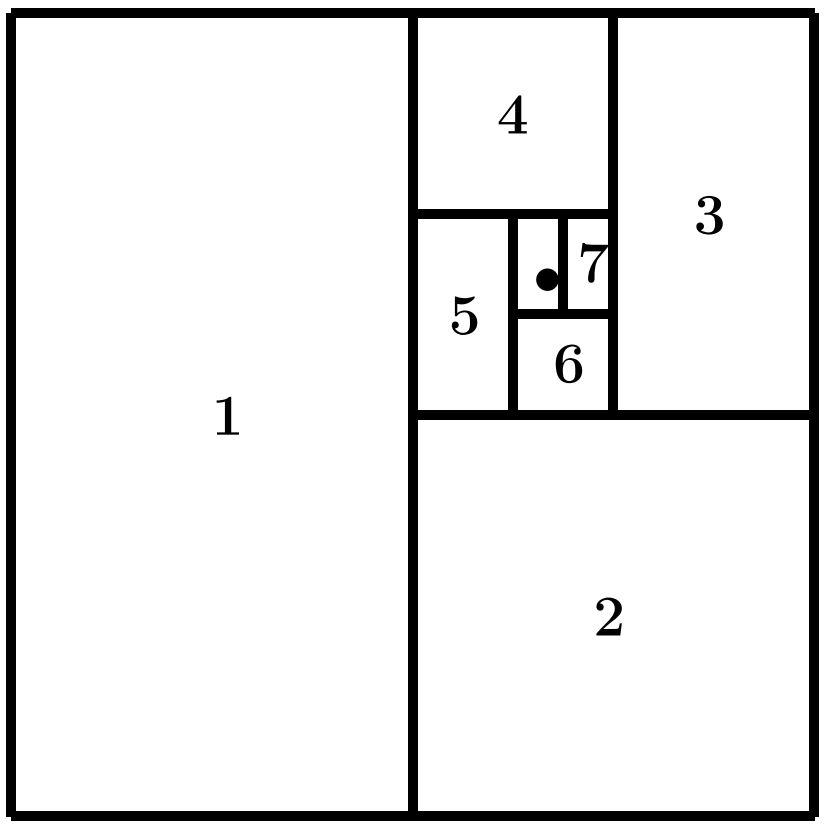
\includegraphics[width=\linewidth]{9D-1}
        \end{figure}
    \end{minipage}
\end{minipage}}
{НаписанноеРешение}
{ВерныйОтвет}{Подсказка}
\end{problem}

\begin{problem}{Геометрическая прогрессия.}{9.6.3}{9D}{*}
{Известно, что для неизвестных $x$ и $y$ верно уравнение $x = y + y^{2} + \ldots + y^{n} + \ldots$\\
Оказывается, можно в таком же виде выразить $x$ через $y$ (представить в виде степенного ряда), то есть $$x = ay + by^{2} + cy^{3} + \ldots$$
Найти этот ряд (его коэффициенты $a$, $b$, $c$, ...)}
{НаписанноеРешение}
{ВерныйОтвет}{Подсказка}
\end{problem}

\begin{problem}{Метод математической индукции.}{9.6.4}{9I}{(лёгкая)}
{Некто разбил координатную плоскость десятками прямых вдоль и поперёк на очень много частей.\\ Правда ли, что полученные части можно раскрасить двумя цветами так, что никакие две части одного цвета не будут граничить друг с другом по стороне?\\ (Общий угол у двух участков одного цвета может быть, общая сторона~--- нет).}
{НаписанноеРешение}
{ВерныйОтвет}{Подсказка}
\end{problem}

\begin{problem}
{Метод математической индукции.}{9.6.4}{9I red вообще-то номер на биективность, но та же бинарная идея раскрашивания}{(лёгкая)}
{На контурной карте России 85 регионов. Вовочка хочет покрасить на карте каждый регион в белый, синий или красный цвет так, чтобы белый и красный цвета не имели общей границы. При этом один или даже два цвета можно не использовать. Доказать, что количество вариантов такой раскраски — нечётно.}
{НаписанноеРешение}
{ВерныйОтвет}{Подсказка}
\end{problem}

\begin{problem}{Метод математической индукции.}{9.6.4}{9I}{(лёгкая)}
{Доказать, что абсолютно любую сумму, большую 4 рублей, можно уплатить монетами по 5 и 2 рубля.}
{НаписанноеРешение}
{ВерныйОтвет}{Подсказка}
\end{problem}

\begin{problem}{Метод математической индукции.}{9.6.4}{9I https://www.problems.ru/view_problem_details_new.php?id=35022}{(лёгкая)}
{$N$ разбойников делят добычу. У каждого из них свое мнение о ценности той или иной доли добычи, и каждый из них хочет получить не меньше, чем $\frac1N$ долю добычи (со своей точки зрения).\\
Придумать алгоритм, как разделить добычу между разбойниками.}
{НаписанноеРешение}
{ВерныйОтвет}{Подсказка}
\end{problem}

\begin{problem}{Метод математической индукции.}{9.6.4}{9I https://www.problems.ru/view_problem_details_new.php?id=73617}{(лёгкая)}
{На кольцевой автомобильной дороге стоят несколько одинаковых автомашин.\\ Если бы весь бензин, имеющийся в этих автомашинах, слили в одну, то эта машина смогла бы проехать по всей кольцевой дороге и вернуться на прежнее место. Доказать, что хотя бы одна из этих машин может объехать всё кольцо, забирая по пути бензин у остальных машин.}
{НаписанноеРешение}
{ВерныйОтвет}{Подсказка}
\end{problem}

\begin{problem}{Метод математической индукции.}{9.6.4}{9I https://www.problems.ru/view_problem_details_new.php?id=65864}{(лёгкая)}
{Сто медвежат нашли в лесу ягоды: самый младший успел схватить 1 ягоду, медвежонок постарше --- 2 ягоды, следующий --- 4 ягоды, и так далее, самому старшему досталось $2^{99}$ ягод. Лиса предложила им поделить ягоды <<по справедливости>>. Она может подойти к двум медвежатам и распределить их ягоды поровну между ними, а если при этом возникает лишняя ягода, то лиса её съедает. Такие действия она продолжает до тех пор, пока у всех медвежат не станет ягод поровну. Какое наибольшее количество ягод может съесть лиса?}
{НаписанноеРешение}
{ВерныйОтвет}{Подсказка}
\end{problem}

\begin{problem}{Метод математической индукции.}{9.6.4}{7A}{(лёгкая)}
{Доказать тождество для всех натуральных $n$: $\;1 + 3 + \ldots + (2n - 3) + (2n - 1) = n^{2}$.}
{НаписанноеРешение}
{ВерныйОтвет}{Подсказка}
\end{problem}

\begin{problem}{Метод математической индукции.}{9.6.4}{10A}{(лёгкая)}
{a) Известно, что для величины $S(n) = 1^{2} + 2^{2} + \ldots + n^{2}$ (суммы квадратов всех чисел от 1 до $n$) существует выражение в замкнутой форме (то есть, без точек).\\ Угадать, что это за выражение.
\\b) Доказать, что эта формула верна для любого $n$.}
{НаписанноеРешение}
{$\frac16 n(n + 1)(2n + 1)$}{Это многочлен третьей степени.}
\end{problem}

\begin{problem}{Метод математической индукции.}{9.6.4}{9I}{(лёгкая)}
{Доказать равенство методом математической индукции: $$\;\displaystyle 1^{2} + 3^{2} + \ldots + (2n - 1)^{2} = \frac{n(2n - 1)(2n + 1)}{3}.$$

}
{НаписанноеРешение}
{ВерныйОтвет}{Подсказка}
\end{problem}

\begin{problem}{Метод математической индукции.}{9.6.4}{9I}{(лёгкая)}
{Доказать равенство методом математической индукции: $$\;\displaystyle 1^{3} + 2^{3} + \ldots + n^{3} = (1 + 2 + \ldots + n)^2.$$}
{НаписанноеРешение}
{ВерныйОтвет}{Подсказка}
\end{problem}

\begin{problem}{Метод математической индукции.}{9.6.4}{9I}{(лёгкая)}
{Доказать равенство методом математической индукции: $$\;\displaystyle 1^{3} + 3^{3} + \ldots + (2n - 1)^{3} = n^{2}(2n^{2} - 1).$$}
{НаписанноеРешение}
{ВерныйОтвет}{Подсказка}
\end{problem}

\begin{problem}{Метод математической индукции.}{9.6.4}{9I}{(лёгкая)}
{Доказать тождество методом математической индукции: $$1\cdot2\cdot3 + 2\cdot3\cdot4 + \ldots + n(n + 1)(n + 2) = \frac14 n(n + 1)(n + 2)(n + 3).$$}
{НаписанноеРешение}
{ВерныйОтвет}{Подсказка}
\end{problem}

\begin{problem}{Метод математической индукции.}{9.6.4}{9I}{(лёгкая)}
{Доказать равенство методом математической индукции: $$\;\displaystyle 1 \cdot 1! + 2 \cdot 2! + 3 \cdot 3! + \ldots + n \cdot n! = (n + 1)! - 1.$$}
{НаписанноеРешение}
{ВерныйОтвет}{Подсказка}
\end{problem}

\begin{problem}{Метод математической индукции.}{9.6.4}{9I}{(лёгкая)}
{Доказать равенство методом математической индукции: $$\frac{1}{4 \cdot 5} + \frac{1}{5 \cdot 6} + \frac{1}{6 \cdot 7} + \ldots + \frac{1}{(n + 3) \cdot (n + 4)} = \frac{n}{4(n + 4)}.$$}
{НаписанноеРешение}
{ВерныйОтвет}{Подсказка}
\end{problem}

\begin{problem}{Метод математической индукции.}{9.6.4}{9I}{(лёгкая)}
{Доказать равенство методом математической индукции: $$\frac{7}{1 \cdot 8} + \frac{7}{8 \cdot 15} + \frac{7}{15 \cdot 22} + \ldots + \frac{7}{(7n - 6) \cdot (7n + 1)} = 1 - \frac{1}{7n + 1}.$$}
{НаписанноеРешение}
{ВерныйОтвет}{Подсказка}
\end{problem}

\begin{problem}{Метод математической индукции.}{9.6.4}{9I}{(лёгкая)}
{Известно, что $x + \frac1x$ --- целое число.\\ Показать, что тогда число $x^n + \frac{1}{x^n}$ --- также целое, при любом целом $n$.}
{НаписанноеРешение}
{ВерныйОтвет}{Подсказка}
\end{problem}

\begin{problem}{Метод математической индукции.}{9.6.4}{9I}{(лёгкая)}
{Доказать неравенство методом математической индукции ($\forall n \in \mathbb{N}$): $$\;\displaystyle \frac{1}{n + 1} + \frac{1}{n + 2} + \ldots + \frac{1}{3n + 1} > 1.$$}
{НаписанноеРешение}
{ВерныйОтвет}{Подсказка}
\end{problem}

\begin{problem}{Метод математической индукции.}{9.6.4}{9I}{(лёгкая)}
{Доказать неравенство для натуральных $n > 1$: $\quad\displaystyle \frac{(2n)!}{(n!)^2} > \frac{4^n}{n + 1}$.}
{НаписанноеРешение}
{ВерныйОтвет}{Подсказка}
\end{problem}

\begin{problem}{Метод математической индукции.}{9.6.4}{9I}{(лёгкая)}
{Доказать неравенство $2^n > \frac{765}{543}n$ для натуральных чисел.}
{НаписанноеРешение}
{ВерныйОтвет}{Подсказка}
\end{problem}

\begin{problem}{Метод математической индукции.}{9.6.4}{9D}{*}
{Доказать неравенство Бернулли: $(1 + a)^n \geqslant 1 + na$, где $a > -1$, $n \in \mathbb{N}$.}
{НаписанноеРешение}
{ВерныйОтвет}{Подсказка}
\end{problem}

\begin{problem}{Метод математической индукции.}{9.6.4}{9I}{*}
{Доказать неравенство методом математической индукции ($\forall n \in \mathbb{N}$): $$\;\displaystyle |\sin nx| \leqslant n|\sin x|.$$}
{НаписанноеРешение}
{ВерныйОтвет}{Подсказка}
\end{problem}

\begin{problem}{Метод математической индукции.}{9.6.4}{9D 1/2+1/2n}{*}
{Пусть $a_1^2$, $a_2^2$, $a_3^2$, ... $a_n^2$ --- квадраты $n$ различных натуральных чисел, больших 1.
$$\text{Докажи, что } \;\left(1 - \frac{1}{a_1^2}\right)\cdot\left(1 - \frac{1}{a_2^2}\right)\cdot\left(1 - \frac{1}{a_3^2}\right)\cdot\ldots\cdot\left(1 - \frac{1}{a_n^2}\right) > \frac12.$$}
{НаписанноеРешение}
{ВерныйОтвет}{Подсказка}
\end{problem}

\begin{problem}{Метод математической индукции.}{9.6.4}{9D}{*}
{Вычислить произведение $\displaystyle\;A(n) = \frac{2^3-1}{2^3+1}\cdot \frac{3^3-1}{3^3+1}\cdot \frac{4^3-1}{4^3+1}\cdot\ldots\cdot \frac{n^3-1}{n^3+1}$.\\
Найти $\displaystyle\lim_{n\to\infty} A(n)$.}
{НаписанноеРешение}
{ВерныйОтвет}{Подсказка}
\end{problem}

\begin{problem}{Метод математической индукции.}{9.6.4}{9I red многопунктовая}{(лёгкая)}
{Доказать методом математической индукции, что для любого натурального $n$
\\a) $\displaystyle 6^{2n - 1} + 1$ кратно 7; \hfill b) $\displaystyle 3^{3n + 2} + 2^{4n + 1}$ кратно 11; \\ c) $\displaystyle 4^{n} + 15n - 1$ кратно 9; \hfill d) $\displaystyle 7^{2n} - 1$ кратно 48.}
{НаписанноеРешение}
{ВерныйОтвет}{Подсказка}
\end{problem}

\begin{problem}{Инварианты.}{9.6.5}{9D}{(лёгкая)}
{Набор чисел $a$, $b$, $c$ каждую секунду заменяется на набор чисел $a + b - c$, $b + c - a$, $c + a - b$. В начале имеется набор чисел $2000$, $2002$, $2003$.\\ a) Может ли через некоторое время получиться набор чисел 1995, 2003, 2007? \\ b) А набор 2001, 2002, 2003?}
{НаписанноеРешение}
{ВерныйОтвет}{Подсказка}
\end{problem}

\begin{problem}{Инварианты.}{9.6.5}{9D}{(лёгкая)}
{В языке древнего племени алфавит состоит всего из двух букв: <<М>> и <<О>>.\\ Два слова являются синонимами, если одно из другого можно получить при помощи исключения или добавления буквосочетаний <<МО>> и <<ООММ>>, повторяемых в любом порядке и любом количестве.\\ Являются ли синонимами в языке древнего племени слова <<ОММ>> и <<МОО>>?}
{НаписанноеРешение}
{ВерныйОтвет}{Подсказка}
\end{problem}

\begin{problem}{Инварианты.}{9.6.5}{9D}{(лёгкая)}
{На доске выписаны числа $1, 2, \ldots, 20$.\\ Разрешается стереть любые два числа $a$ и $b$ и заменить их на число $ab + a + b$.\\ Какое число может остаться на доске после 19 таких операций?}
{НаписанноеРешение}
{ВерныйОтвет}{Подсказка}
\end{problem}

\begin{problem}{Инварианты.}{9.6.5}{9D}{(лёгкая)}
{На острове Серобуромалин живёт 13 серых, 15 бурых и 17 малиновых хамелеонов. Когда встречаются два хамелеона разного цвета, они одновременно перекрашиваются в третий цвет. Если все хамелеоны станут одного цвета, наступит конец света. Доказать, что конец света не наступит.}
{НаписанноеРешение}
{ВерныйОтвет}{Подсказка}
\end{problem}

\begin{problem}{Инварианты.}{9.6.5}{9D}{*}
{Поле представляет собой клетчатый квадрат $12 \times 12$, в одной из клеток которого находится замаскированный танк. Истребитель за один выстрел обстреливает одну клетку. Если произошло попадание, танк переползает на соседнюю по стороне клетку поля, если нет~--- остаётся на месте.\\ При этом после выстрела пилот истребителя не знает, произошло ли попадание.\\ Для уничтожения танка надо попасть в него два раза. Каким наименьшим числом выстрелов можно обойтись для того, чтобы гарантировать, что танк уничтожен?

}
{НаписанноеРешение}
{ВерныйОтвет}{Подсказка}
\end{problem}

\begin{problem}{Инварианты.}{9.6.5}{9D}{*}
{В одной из вершин шестиугольника лежит золотая монета, а в остальных ничего не лежит. Кощей Бессмертный чахнет над златом и каждое утро снимает с одной вершины произвольное количество монет, после чего тут же кладёт в соседнюю вершину в шесть раз больше монет. Если к концу какого-то дня во всех вершинах будет поровну монет, Кощей станет Властелином Мира. Доказать, что хоть злата у него и сколько угодно, но Властелином Мира Кощею не бывать.}
{НаписанноеРешение}
{ВерныйОтвет}{Подсказка}
\end{problem}

\begin{problem}{Инварианты.}{9.6.5}{9D}{*}
{Тимофей резал ножницами лист бумаги (обычный прямоугольный лист размера А4) на кусочки. Все разрезы прямые.\\ Сначала он разрезал этот прямоугольник на две части. Потом разрезал на два куска одну из полученных частей, и так далее. Когда ему надоело резать, оказалось, что общее количество углов у всех получившихся фигур равно 2020.\\ Сколько разрезов мог сделать Тимофей? Выбери все верные ответы.\\
(A) 2020\hfill(B) 2016\hfill(C) 1009\hfill(D) 670\hfill(E) 503}
{НаписанноеРешение}
{ВерныйОтвет}{Подсказка}
\end{problem}

\end{document}